\documentclass[11pt]{amsart}

%------------------Packagages------------------------------

\usepackage[a4paper, margin=2.5cm]{geometry}
\usepackage{amsmath, amsthm, amssymb, mathtools}
\usepackage{graphicx}
\usepackage{booktabs}
\usepackage[hyphens]{url}
\usepackage{natbib}
\usepackage{hyperref}
\hypersetup{
    colorlinks = true,
    urlcolor   = blue,
    citecolor  = black,
}
\usepackage{upref}
\usepackage{siunitx}

%------Theorem Environment----------

% This environment is based on Anna Marie Bohmann's template, which in turn is based on Peter May's REU latex template
% Anna Marie Bohmann's template: https://math.vanderbilt.edu/bohmanar/latex.html
% University of Chicago's REU program: http://math.uchicago.edu/~may/REU2024/
% These take care of numbering of theorems and lemmas automatically
%theoremstyle{plain} --- default
\newtheorem{thm}{Theorem}[section]
\newtheorem{cor}[thm]{Corollary}
\newtheorem{prop}[thm]{Proposition}
\newtheorem{lem}[thm]{Lemma}

\theoremstyle{definition}
\newtheorem{defn}[thm]{Definition}
\newtheorem{exmp}[thm]{Example}
\newtheorem{notn}[thm]{Notation}

\theoremstyle{remark}
\newtheorem{rem}[thm]{Remark}

\makeatletter
\let\c@equation\c@thm
\makeatother
\numberwithin{equation}{section}

%---------------------------Information------------------------------

\title{The Fast Fourier Transform}
\author{Adithya Nair, Kausik Muthukumar, P Ananthapadmanabhan Nair, Srujana Duvvuri}
\date{May 2024}

%--------------------------------------------------------------------

\begin{document}
\begin{abstract}
	This report aims to extend an understanding of the Fourier Series and the Fourier Transform into the Fast Fourier Transform algorithm. The report goes over the mathematical basis behind the algorithm as well as its implementation and widespread use in the world today. The report will also demonstrate the algorithm through a computational problem.
\end{abstract}

\maketitle

\section{Introduction}\label{sec1}
This report  

\section{Discrete Fourier Analysis}
Fourier analysis decomposes the sampled signal into its fundamental periodic constituents or complex exponential constituents. Each exponential constituent together, forms an infinite orthogonal basis. Functions are expressed in infinite dimensional spaces, a Fourier series of a given function gives us an orthogonal basis to express that same function which is convenient for differentiation and integration.

\begin{align*}
	&x_j = a + jh, \ j = 0, \dots, n, & \text{where} \ h = \frac{b-a}{n}
\end{align*}

In signal processing, $x$ represents time instead of space, $x_j$ represents the times we sample $f(x)$.

We use $0 \leq x \leq 2 \pi$ with n equally spaced points,(any function outside that can simply be rescaled.)
\[ 
	x_0 = 0, x_1 = \frac{2\pi}{n}, x_2 = \frac{4\pi}{n}, x_j = \frac{2j\pi}{n}, x_{n-1} = \frac{2(n-1)\pi}{n}
\]

An important consequence of sampling is that it cannot distinguish between values that have the same values at all sample points.
Take for example, $e^{inx}$

\[
	f(x) = e^{inx} = \cos{nx} + i \sin{nx}
\]


The discrete Fourier representation, has sampled values,

\[
	f_j = f(\frac{2j \pi}{n}) = exp(in \frac{2j\pi}{n}) = e^{2j\pi i} = 1
\]

What this means is that sampling at n equally spaced samples \textbf{cannot} detect periodic signals of $n$ frequency. The Fourier representation always gives the same sample vector $(1,1,\dots, 1)^T$. 

Then the complex functionals for the sample points,
\begin{equation}
\label{epower}e^{i(k+n)x} = e^{ikx}
\end{equation}



So we need to only use the first $n$ periodic complex exponential functions. Anything above that does not yield any use for a function with $n$ sample points.

Negative frequencies can be converted into positive frequencies by adding $n$

\begin{equation}
	e^{-ikx} = e^{i(n-k)x} \label{negativefreq}
\end{equation}

The discrete fourier representation of a function $f(x)$ decomposes a sampled function into a linear combination of complex exponentials. This representation does not need to go past $e^{n-1}$, (See \ref{epower})

\begin{equation}
	f(x) \sim p(x) = c_0 + c_1 e^{ix} + c_2 e^{2ix} + \cdots + c_{n-1}e^{(n-1)ix}
	\label{repcomp}
\end{equation}
\begin{rem}
	If $f(x)$ is real then $p(x)$ is real, at the sampled points, but the function could be complex in between. The imaginary component of the function is removed and $p(x)$ is treated as the interpolating trigonometric polynomial of the function $f(x)$. But, the representation is still retained for convenience.
\end{rem}

Writing this in a vector form that belongs in $\mathbb{C}^n$, For each sampled value, we get a vector $\vec{\omega_k}$, which is the vector of all the complex exponentials with the sampled values of $x$ for a given frequency $k$, $0 < k < n$
\begin{align*}
	\omega_k &= [e^{i k x_0},e^{ik x_1},\cdots,e^{ik x_{n-1}}]^T \\
	\omega_k &= [1,e^{i k \frac{2\pi}{n}},e^{ik \frac{4\pi}{n}},\cdots,e^{ik \frac{2\pi(n-1)}{n}}]^T \\
\end{align*}

Upon applying what we know of the function,
\[
	f(x_j) = p(x_j)
\]
We can write the entire function sample vector as a finite linear combination of the complex exponentials with coefficients $c_k$ for each sampled value.
\begin{equation}
	\vec{f} = c_0 \omega_0 + c_1 \omega_1 + \cdots c_{n-1} \omega_{n-1}
	\label{complexeform}
\end{equation}

To find the coefficients, we need to simply apply an inner product, to isolate each term and find these coefficients.

For vectors in $\mathbb{C}^n$, we define the inner product as,

\[
	\langle f,g \rangle = \frac{1}{n} \sum_{j = 0}^{j = n-1} f_j \overline{g_j} = \frac{1}{n} f(x_j) \overline{g(x_j}
\]

To prove Theorem \ref{orthonormalbasis}, we need to understand the properties of $n^{th}$ roots of unity.

\subsection{Nth Roots Of Unity}
\begin{defn}
A number $z$ satisfying the equation, where $n \in Z^+$,
\[
	z^n = 1
\]
\end{defn}
We define, 
\[
	\zeta_n = e^{2 \pi i/n}
\]

Where,
\[
	\zeta_n^n = e^{(2 \pi i / n)n} = 1
\]

Which means that,

\[
	\zeta_n = \sqrt[n]{1}
\]

Also, any $k^{th}$ power of $\zeta_n$ is also an $n^{th}$ root of unity

\[
	(z^k)^n = (z^n)^k = 1^k = 1
\]

So for the polynomial $z^n - 1$,

\[
		z^{n}-1 = (z-1)(z -  \zeta_n)(z-\zeta_n^2)\cdots(z - \zeta_n^{n-1}) 
\]

Onto proving that this linear combination has an orthonormal basis, upon proving this, the Fourier Transform shifts from a mathematical toy into one of the most powerful algorithms ever discovered.
\pagebreak
\begin{thm} \label{orthonormalbasis}
	The sampled exponential vectors $\omega_0, \cdots , \omega_{n-1}$ form an orthogonal basis in $\mathbb{C}^n$ with respect to the inner product,
	\[
		\langle f,g \rangle = \frac{1}{n} \sum_{j=0}^{n-1} f_j \overline{g_j}
	\]
\end{thm}
\begin{proof}
Take $\zeta_n^k = e^{\frac{2\pi k i}{n}}$, this means that $\zeta^n_n = 1$, and there are n equally spaced such complex numbers, between $\zeta_1$ and $\zeta_n$. This means that $\zeta_k$ and all powers of $\zeta_k$ act as $n^{th} $roots of unity

	\begin{align}
		z^{n}-1 &= (z-1)(z -  \zeta_n)(z-\zeta_n^2)\cdots(z - \zeta_n^{n-1}) &\text{(Since they're $n^{th}$ roots of unity})  \label{pf1} \\
		z^n-1 &= (z-1)(1 + z + z^2 + \cdots + z^{n-1}) &\text{(Through algebraic factorization)} \label{pf2}
	\end{align}
	We equate the two to get,
	\begin{align*}
	(z-1)(1 + z + z^2 + \cdots + z^{n-1})  &= (z-1)(z -  \zeta_n)(z-\zeta_n^2)\cdots(z - \zeta_n^{n-1}) \\
	1 + z + z^2 + \cdots + z^{n-1}  &= (z -  \zeta_n)(z-\zeta_n^2)\cdots(z - \zeta_n^{n-1}) \\
		1 + \zeta_n^k + \zeta_n^{2k} + \cdots + \zeta_n^{(n-1) k} &= \{n,k = 0 \text{ and } 0, 0 < k < n \} \\
	\end{align*}
As a consequence of \ref{epower}, this extends to all integers $n$. If k is a multiple of n, then the sum gives n, and 0 for all other values of k.

Writing the sampled exponential vectors in terms of the $n^{th}$ roots of unity,

\[
	\omega_k = (1, \zeta_n^k, \zeta_n^{2k},\zeta_n^{3k}, \cdots, \zeta_n^{(n-1)k})^T
\]

We conclude that, 
\[
	\langle	\omega_k, \omega_l \rangle = \frac{1}{n} \sum_{j=0}^{n-1} \zeta_{n}^{jk} \overline{\zeta_{n}^{jl}} = \frac{1}{n} \sum_{j=0}^{n-1} \zeta_n^{j(k-l)} = \{1, k = l \text{ and } 0, k \neq l\}
\]
\end{proof}

Now that orthonormality is established, we can now isolate each discrete Fourier coefficient and compute them by applying inner products.

The properties of an orthonormal basis allows us to isolate any given component $v_i$ of the vector $\vec{v}$ by simply performing the inner product of $\vec{q_i}$ with the vector $\vec{v}$
\begin{align*}
	\vec{q_i}^T\vec{v} &= \vec{q_i}^T v_1 \vec{q_1} + \vec{q_i}^T v_2 \vec{q_2} + \cdots + \vec{q_i}^T v_i \vec{q_i} + \cdots + \vec{q_i}^T v_n \vec{q_n} \\
	\vec{q_i}^T \vec{v} &= v_i &(\vec{q_i}\cdot \vec{q_j} = 0, \vec{q_i} \cdot \vec{q_i} = 1)
\end{align*}


So to compute a discrete Fourier coefficient $c_k$,

\[
	c_k = \langle f, \omega_k \rangle = \frac{1}{n} \sum_{j=0}^{n-1} f_j \overline{e^{ikx_j}} = \frac{1}{n} \sum_{j=0}^{n-1} \zeta_n^{-jk} f_j
\]

In a way we are averaging the sampled values of the product of $f(x) e^{-ikx}$

From this computation, we finally arrive at the Discrete Fourier Transform

\begin{defn}
The passage from a signal to its Fourier coefficients is known as The \textbf{Discrete Fourier Transform}
\end{defn}


\begin{defn}
The reconstruction of a signal from its Fourier coefficients is known as the \textbf{Inverse Discrete Fourier Transform}
\end{defn}

This is done using equations \ref{complexeform} and \ref{repcomp}.
\subsection{Computing Coefficients Using Matrices }
We can express this computatoin through a matrix multiplication.

For a given Fourier coefficient,

\[
	{c}_k = \frac{1}{n}\sum_{j=0}^{n-1} f_j \zeta_n^{-jk}
\]

So we can construct a Vandermonde matrix $F_n$ where a given term $a_{ij} = \zeta_n^{ij}$, where $i,j = 0, \cdots, {n-1}$

\begin{equation}
	\begin{bmatrix}
		c_{0} \\
		c_{1} \\
		c_{2} \\
		\vdots \\
		c_{n-1} 
	\end{bmatrix}
	=
	\begin{bmatrix}
		1 & 1 & 1 & \cdots & 1 \\
		1 & \zeta_n & \zeta_n^2 & \cdots & \zeta_n^{n-1} \\
		1 & \zeta_n^2 & \zeta_n^4 & \cdots & \zeta_n^{2(n-1)} \\
		\vdots & \vdots & \vdots & \ddots & \vdots \\
		1 & \zeta_n^{n-1} & \zeta_n^{2(n-1)} & \cdots & \zeta_n^{(n-1)^2}
	\end{bmatrix}
	\begin{bmatrix}
		f_0 \\
		f_1 \\
		f_2 \\
		\vdots \\
		f_{n-1}
	\end{bmatrix}
	\label{matrixFourier}
\end{equation}
This matrix $F_n$ is Hermitian.

\subsection{Reducing high frequency oscillatory terms}
If we look at the expression for the discrete Fourier representation of a given function, the complex exponentials quickly tend to very high frequencies. Graphically showing the consequences of this, 

Let's take $f(x) = \sin(x)$,


\begin{figure}[!ht]
    \centering
    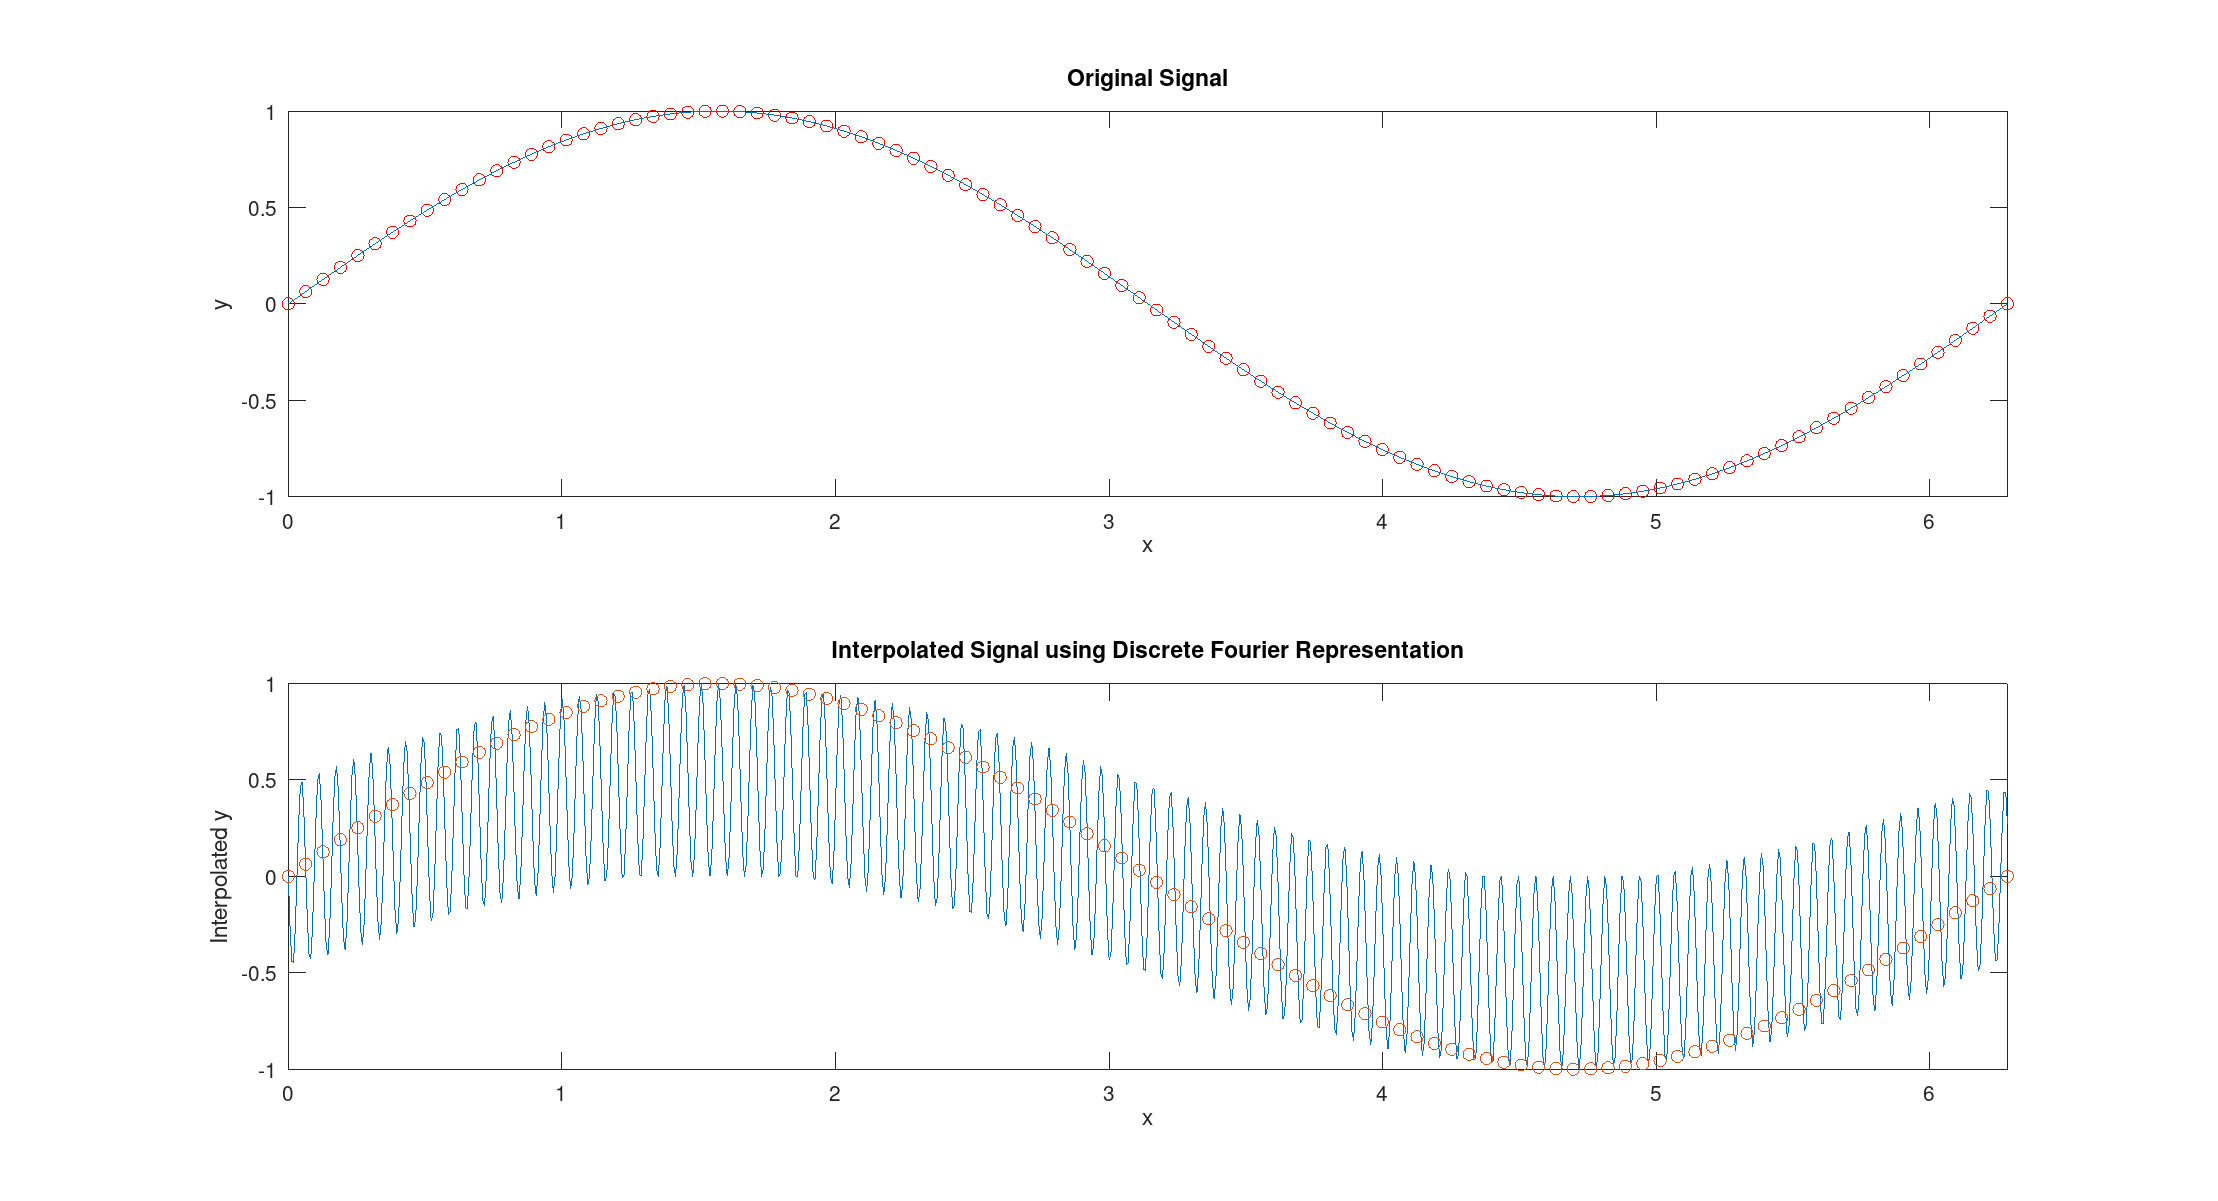
\includegraphics[trim = 0 250 0 250, width=\linewidth,clip]{plots/interpolation.pdf}
    \caption{Comparison of original signal and interpolated signal}
    \label{fig:dft_interpolation}
\end{figure}

For a given function,


See \ref{fig:dft_interpolation}, the function is correct at all sampled points.
But it varies widely at all other points. Which isn't very useful when trying to approximate functions.

The solution to this is to take the series a bit differently. Instead of taking the complex exponentials, $\zeta_n^0$ to $\zeta_n^{n-1}$, we take,

For interpolation purposes, we change the complex exponentials to lower frequency equivalents using the consequences of Equation \ref{epower} or more precisely \ref{negativefreq}.

This is convenient because we don't have to recompute the Fourier coefficients when we change the complex exponentials since,

So if n is odd, $m = \frac{n-1}{2},$

\[
	\hat{p}(x) = c_{-m} e^{-imx} + \cdots + c_{-1} e^{-ix} + c_0 + c_1e^{ix} + \cdots + c_me^{imx} = \sum_{k = -m}^{m} c_k e^{ikx}
\]

And if n is even, $m = \frac{n}{2},$

\[
	\hat{p}(x) = c_{-m} e^{-imx} + \cdots + c_{-1} e^{-ix} + c_0 + c_1e^{ix} + \cdots + c_me^{i(m-1)x} = \sum_{k = -m}^{m-1} c_k e^{ikx}
\]

We write the corresponding Fourier coefficients as,

\[
	c_{-k} = c_{n-k}
\]

We can do this since, we know that the corresponding inner products for the Fourier coefficients are equal.

TODO: INSERT COMPARISON FIGURE HERE[written using OCTAVE]

Thus we get an interpolated function that does not oscillate as wildly as the original discrete Fourier representation where k went from $0$ to $n-1$


\section{Properties Of The Fourier Transform}
\subsection{Linearity of the DFT}
Suppose if we have an input signal x(n) undergoing a Fourier transform $(F)(x_n) = X_k$ and another input  signal y(n) $(F)(y_n) = Y_k$ then for any complex number a and b the  Fourier transform of the linear combination of these complex numbers with the input signals , 
\[(F)(ax_n + by_n) = aX_k + bX_k\]

\subsection{Periodicity}
The DFT always assumes a given signal is periodic in nature with a period N with only the discrete frequencies. 

\subsection{Time and Frequency Reversal}
Reversing the time domain i.e replacing n with N-n corresponds to reversing in the frequency domain i.e replacing k with N-k where N is the period of the input sample.
Mathematically ,
\[(F)(x_n) = X_k \] then , 
\[(F)(x_(N-n) = X_(k-n)\]

\subsection{Parseval's Theorem and Plancherel Theorem}
This theorem asserts that the Fourier Transform is unitary and therefore preserves the inner product between two functions. In this context , if we have two input signals $x_n$ and $y_n$ and their respective DFT outputs $X_k$ and $Y_k$ then the theorem is , 
\[\sum_{n = 0}^{N-1} x_n y_n^{*} = \sum_{n=0}^{N-1} X_k Y_k^{*}\]
where "*" denotes the complex conjugate of the input.

Plancherel Theorem is a special case of the Parsevals theorem which states,
\[\sum_{n = 0}^{N-1} \mod{ x_n^2} = \sum_{n=0}^{N-1} \mod{ X_k^2}\]

\subsection{Shift property}
The shift property states that the DFT of the shifted signal y[n] is equal to the DFT of the original signal x[n] multiplied by a complex exponential term that represents a phase shift. Mathematically, it can be expressed as:
\[Y(k) = X(K) \cdot e^{\frac{-j2 \pi k m}{N}}\]
Where , 
Y[k] is the DFT of the shifted signal y[n].
X[k] is the DFT of the original signal x[n].
\[e^{\frac{-j 2 \pi km}{N}}\] represents a complex exponential term, which introduces a phase shift in the frequency domain.

\subsection{Complex Conjugate Property}
If x(n) represents a complex input sequence  and the Fourier transform is X(k) then, 
\[\textit{F}(x^{*}(n)) = X^{*}(-k) = X*(N-k)\]

\subsection{Convolution Theorem}
If we have an input signal x(n) and its corresponding Fourier Transformed output X(k) and another input signal h(n) and its Fourier Transformed output H(k) then

\[x(n) \ast h(n)  = X(k) \cdot H(k)\]

Where $\ast$ denotes a convolution which is defined as the inverse Fourier Transform of the two input samples 

\[(u \ast v)(n) = \textit{F}^{-1} (u \cdot v)\]
Which means that the convolution in the time domain represents a multiplication in the frequency domain.


\section{Fast Fourier Transform}
Despite the orthogonality of the Fourier representation, there are limitations to the Discrete Fourier Transform. For an $n$ times sampled signal, $n^2$ complex multiplications and $n^2 - n$ complex additions must be performed.

The Discrete Fourier Transform algorithm has a time comlexity $O(n^2)$.

In the early 1960s, James Cooley and John Tukey discovered a much more efficient method for the Discrete Fourier Transform. This algorithm takes advantage of a property of the sampled exponential vectors.

The basic idea behind the Fast Fourier Transform is that if the number of sample points we take is some power of 2 and upon reordering the even and odd sample vectors, then we can write the matrix equation \ref{matrixFourier} as,

\[
	\hat{f} = F_{2^n} \vec{f} = \begin{bmatrix}
		I_{2^{n-1}} & -D_{2^{n-1}} \\
		I_{2^{n-1}} & -D_{2^{n-1}} \\
	\end{bmatrix}
	\begin{bmatrix}
		F_{2^{n-1}} & 0 \\
	0 & F_{2^{n-1}}
	\end{bmatrix}
	\begin{bmatrix}
		f_{even} \\
		f_{odd} \\
	\end{bmatrix}
\]

Where I is the Identity matrix, and D is the diagonal matrix,

\[
	D_{2^{n-1}} = \begin{bmatrix}
		1 & 0 & 0 & \cdots & 0 \\
		0 & \zeta_{2^{n-1}} & 0 &\cdots & 0\\
		0 & 0 & \zeta_{2^{n-1}}^2 & \cdots & 0 \\
		\vdots & \vdots & \vdots  &  \ddots & \vdots \\
		0 & 0 & 0 & 0 & \zeta_{2^{n-1}}^{2^{n-1}}
	\end{bmatrix}
\]

This algorithm works by iteratively breaking up each $F_k$ matrix and rearranging the even and odd vectors into this form, until we get a $2\times 2$ $F_2$ matrix

This gives us an algorithm of time complexity $O(n \log{n})$ The $n$ comes from the diagonal matrices 

\begin{rem}
	If the number of sample points is not a power of 2, we can simply add zeros to the vector to make $n = 2^{k}$
\end{rem}

\section{Applications Of The Algorithm}
\subsection{Signal Processing}
When working with any kind of signal processing, it is important to approximate the Fourier transform on discrete vectors of data. However, while the DFT had proved to be very useful in numerous approximations and computations, it did not scale well to very large $n>>1$, due to its requirement of $O(n^2)$ operations. To solve this problem, a fast Fourier transform algorithm that scales $O(nlog(n))$ was created to ensure that as the n becomes very large the $log(n)$ component grows slowly and the algorithm approaches a linear scaling. The fast $O(nlog(n))$ scaling is what enables the use of FFT (fast Fourier transform) in signal processing such as real-time communication, audio and image compression among others.
\subsection {Definition of fast Fourier and Inverse fast Fourier Transform}

For a square image of size $N*N$, the two dimensional FFT is given by:


\[
F(k,l) = \sum_{i=0}^{N-1} \sum_{j =0}^{N-1} f(i,j) e^{-i2\pi(\frac{ki}{N} +\frac{lg}{N}})
\]

In a similar way, the Fourier image can be re-transformed to the domain. The inverse Fourier transform is given by:

\[
	f(a,b) = \frac{1}{N^{2}} \sum_{i=0}^{N-1} \sum_{j =0}^{N-1} F(k,l) e^{-i2\pi(\frac{ki}{N} +\frac{lg}{N}})
\]

\subsection {Image Compression}
In the case of image processing, we will consider a two-dimensional Fourier Transform. A 2-dimensional Fourier transform is achieved by first applying a 1-dimensional fast Fourier transform to every row of the matrix and repeating the same with every column of the matrix. This produces an image shown in figure 1.
\begin{figure} [h]
    \centering
    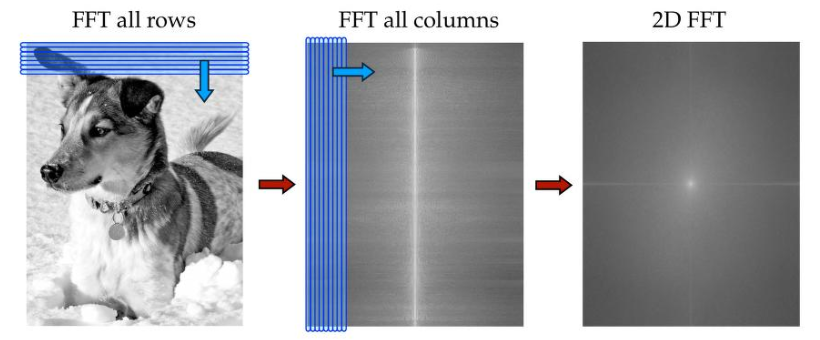
\includegraphics[width=0.5\linewidth]{../pictures/Screenshot 2024-05-22 111943.png}
    \caption{2-dimensional FFT}
    \label{fig:1.1}
\end{figure}

Most of the Fourier coefficients on the image are really small when a Fourier transform is applied. This allows us to discard all the coefficients that are negligible or close to zero and only keep the ones with large enough values, ensuring that there is very little loss in the original image when you apply inverse Fourier transform mentioned above. This allows you to compress the image to the size you want by removing the corresponding number of Fourier coefficients. The quality of the compressed image depends on the number of largest Fourier coefficients kept in the image. 

Figure 2 below, shows the previous image with various thresholds to keep 5, 1 and 0.2 percents of the largest Fourier coefficients.
 \begin{figure} [h]
     \centering
     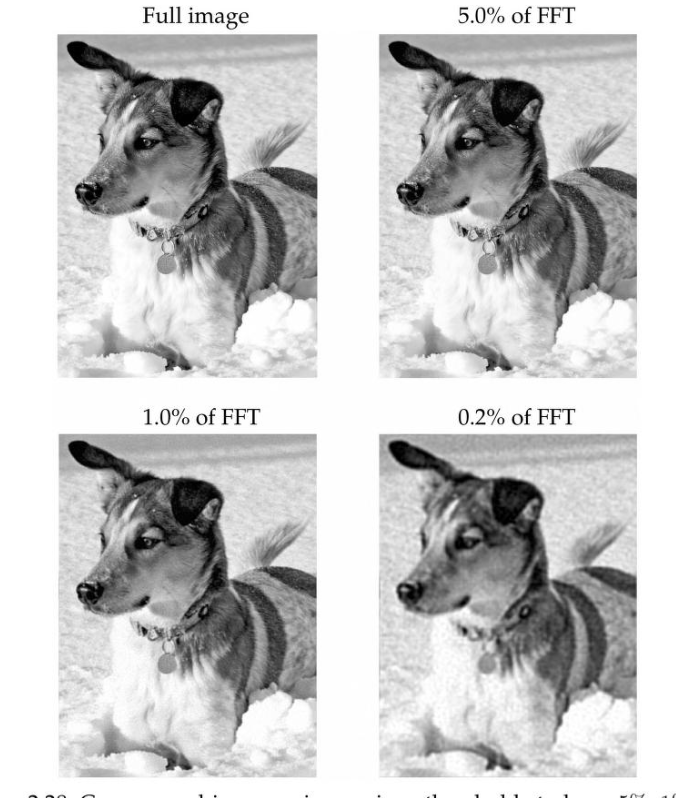
\includegraphics[width=0.5\linewidth]{../pictures/Screenshot 2024-05-22 122030.png}
     \caption{Compressed images} \label{fig:2}
 \end{figure}

 \subsection{Denoising of Data} 
 The denoising of data is an important tool used in several fields ranging from solving PDE's to satellite communication. 

 To efficiently denoise data(refer to figure 3), the noisy signal should first be computed to the fast Fourier transform(top), The power spectral density (PSD) is the normalized squared magnitude of $\hat{f}$ and indicates how much power the signal contains in each frequency(middle). 
\begin{figure}[t]
    \centering
    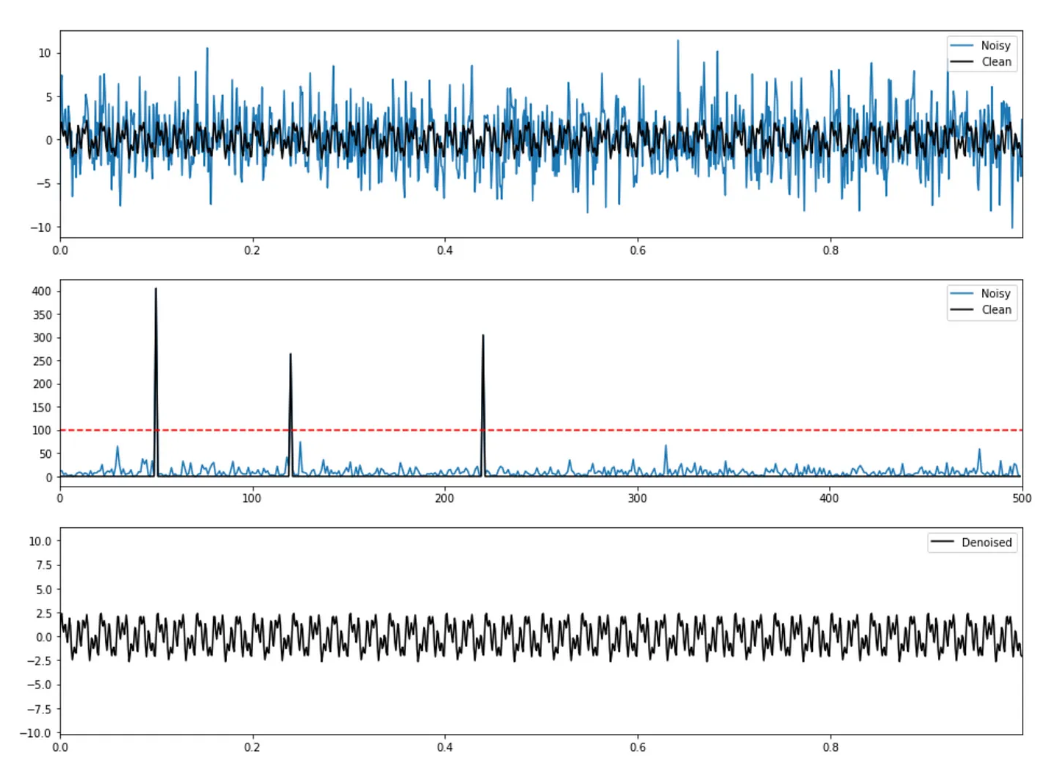
\includegraphics[width=0.5\linewidth]{../pictures/Screenshot 2024-05-22 133404.png}
    \caption{denoising data}
    \label{fig:3}
\end{figure}

It is possible to zero-out components that have power below a threshold to remove noise from the signal. After inverse transforming the filtered signal, we find the clean and filtered time series match quite well(bottom).

\section{Conclusion}


\section*{Acknowledgements}

\appendix

\section{Appendix A: Plotting The Interpolated Signal}\label{appA}

\bibliographystyle{jfm}
\bibliography{references}
\cite{Olver2015TopicsIF}
\cite{Brunton_Kutz_2022}
\cite{Strang2019}
\end{document}
